\documentclass[12pt]{article}

\usepackage{amsmath, amsfonts, amssymb, amsthm, bbm, mathtools}
\usepackage{booktabs, fancyhdr, verbatim, graphicx, float, url}
\usepackage{algorithm}
\usepackage{algpseudocode}
\newenvironment{claim}[1]{\par\noindent\underline{Claim:}\space#1}{}
\newenvironment{claimproof}[1]{\par\noindent\underline{Proof:}\space#1}{\hfill $\blacksquare$}

\title{Final Project Report: QR Factorization on GPUs}
\author{Ryan Synk}

\begin{document}

\maketitle

\section*{Introduction}

This report outlines my work on implementing a fast QR factorization algorithm on a Graphics
Processing Unit (GPU). It closely follows a 2009 paper of Kerr et. al 
\cite{10.1145/1513895.1513904} and focuses on writing code to mimic the results found
in the paper.

\subsection*{Graphics Processing Units}

Graphics processing units (GPUs) are parallel processors initially designed for computing shaders
in computer graphics applications. In a Central Processing Unit (CPU), one large, powerful chip 
performs the computations. GPUs, on the other hand, consist of many small processing units, 
each capable of performing computations in parallel with one another. These small processing
units are referred to by NVIDIA, a GPU manufacturer, as Streaming Multiprocessors (SMs). 
Associated with each SM is a store of L1 cache memory. Each SM, in turn, can access a global 
L2 memory cache --- see figure \ref{fig:gpudiagram} for a diagram of a recent GPU. This 
architecture, with its combination of parallel processors and memory hierarchy, lends 
itself well to fine-grained parallelization --- and in the case of computer graphics, dense 
linear algebra calculations.

\begin{figure}[H]
    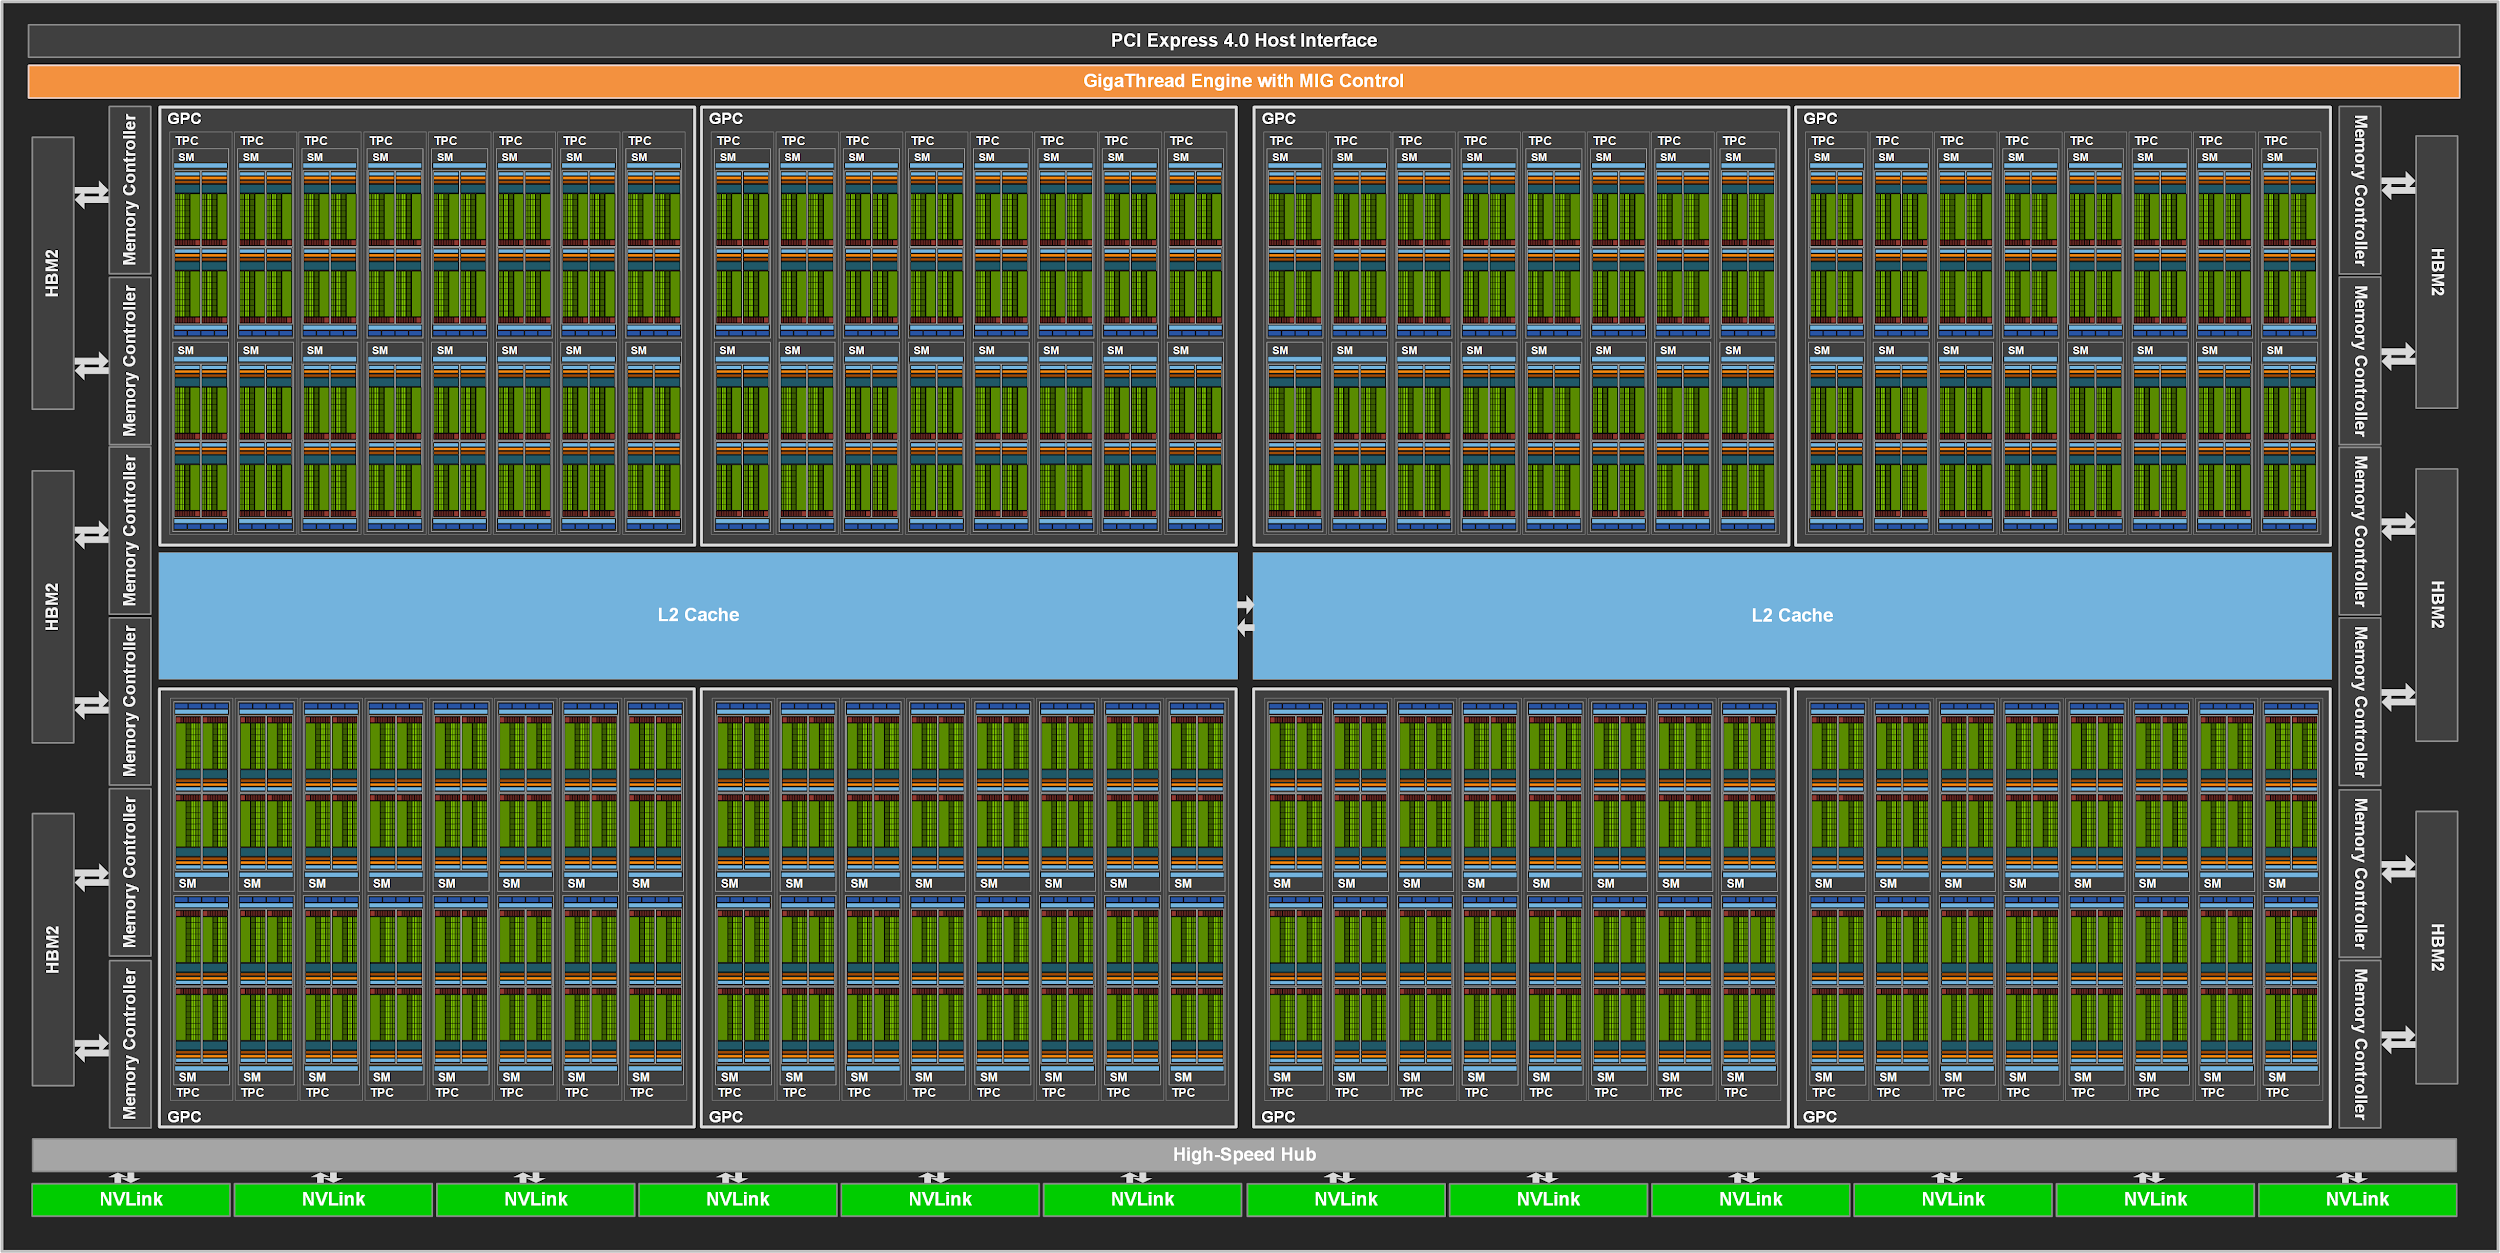
\includegraphics[scale=0.20]{gpu_diagram}
    \caption{NVIDIA Volta GPU. Source: \cite{volta_blogpost}}
    \label{fig:gpudiagram}
\end{figure}

Shortly after the advent of modern graphics processing units with programmable shaders, 
studies in the use of GPUs for scientific computing problems were conducted. In 2001, 
researchers implemented the first matrix-matrix multiplication algorithm for a GPU 
\cite{10.1145/582034.582089}. Eventually, certain applications running on GPUs began to 
outperform their counterparts on CPUs. In a 2005 paper (whose authors include UMD 
Professor Dinesh Manocha), a GPU implementation of LU factorization with partial 
pivoting was shown to outperform a CPU. \cite{1559955}. Scientific computing wasn't the only
field impacted by GPUs.

The training of deep neural networks is a process which involves large amounts of dense
matrix-vector and matrix-matrix multiplications. The discovery that GPUs are well-suited 
to accelerate this traning process was instrumental in the revolution of deep learning 
in the 2010s, helping to turn neural networks from theoretical curiosities into the 
ubiquitous and powerful models they are today.

Work still continues as researchers in numerical linear algebra and high-performance 
computing try to find ways that GPUs can accelerate their algorithms. High-performance 
computing systems are being built with more and more GPU accelerators in them, 
and the DOE's newest exascale supercomputer, Frontier, will be built with four times 
as many GPUs as CPUs \cite{frontier}.

\subsection*{QR Factorization}

In this report, we will develop a GPU-based method to solve the problem of factorizing 
an $m \times n$ matrix $A$ as the product $A = QR$. Here, $Q \in \mathbb{R}^{m \times m}$ 
is an $m \times m$ unitary matrix, and $R$ is an upper-triangular matrix. A number of basic
algorithms for finding such a decomposition exist, and they all follow the pattern of
successively zeroing out entries of $A$ below the main diagonal using unitary transformations.
These methods include

\begin{enumerate}
    \item Givens rotation factorization
    \item Gram-schmidt factorization
    \item Householder QR factorization
\end{enumerate}

For the latter, a series of Householder transformations are used to zero out entries 
below the diagonal of $A$. Given a vector $x \in \mathbb{R}^{n}$, a Householder matrix $P_x$ 
can be generated such that $P_x x = \|x\|e_1$ --- in other words, the matrix transforms
the vector $x$ into a multiple of the $1^{st}$ basis vector in $\mathbb{R}^{n}$.

The transformation $P_x$ is of the form
\begin{flalign*}
    P_x &= I - \frac{2}{v^{T}v}v v^{T} \\
    v &= x - \|x\|e_1
\end{flalign*}

If we choose $x_k$ to be the the vector in $\mathbb{R}^{n - k}$ consisting of entries of the
$k^{th}$ column of $A$, starting at the diagonal and moving downwards ($A(m:k, n)$ in 
MATLAB notation) we can create a householder transformation $P_k$ which zeros out the 
entries below the diagonal of the  $k^{th}$ column of $A$. See figure \ref{fig:householder_qr}
for a diagram.

\begin{figure}[H]
    \centering
    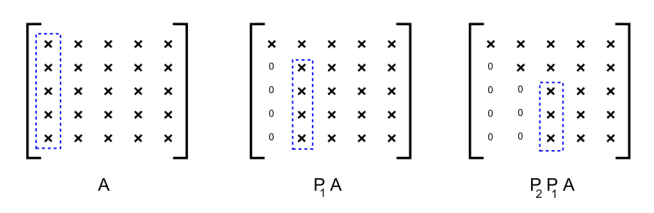
\includegraphics[scale=0.5]{qr_diagram}
    \caption{Successive householder transformations acting on $A$ Source: \cite{10.1145/1513895.1513904}}
    \label{fig:householder_qr}
\end{figure}

Importantly, the $P$ matrices don't need to be fully formed. If we define $\beta_k = \frac{2}{v_k^{T}v_k}$, then
\begin{flalign*}
    PA &= (I - \beta_k v_k v_k^{T}) A \\
    &= A - \beta_k v_k (A^{T} v_k)
\end{flalign*}

So we can perform a rank-one update to $A$ at each iteration.

Putting this together gives the following $QR$ algorithm:

\begin{algorithm}
\caption{QR Factorization Via Householder}\label{alg:cap}
\begin{algorithmic}
\State Given $A\in\mathbb{R}^{mxn}$
\State $Q \gets I_m$ 
\State $R \gets A$
    \For{$k = 1:n$}
    \State $[v, \beta] = \mathbf{house}(R[k:m, 1:n])$ 
    \State $R[k:m, 1:n] = R[k:m, 1:n] - \beta v v^{T} R[k:m, 1:n]$
    \State $Q[1:m, k:m] = Q[1:m, k:m] - \beta Q[1:m, k:m]v v^{T}$
    \EndFor
\end{algorithmic}
\end{algorithm}

This $QR$ algorithm works well, but for our purposes it will require some modification
to run quickly on a GPU.
\par\null\par
TODO:
\begin{enumerate}
    \item Explain how to update Q in basic QR
    \item Explain how chaining together $P$ matrices gives $QR$ 
\end{enumerate}

\section*{Algorithm}
\begin{enumerate}
    \item Explanation of why regular QR doesn't work as well (maybe cite a figure)
    \item Explanation of block QR update (W, Y matrices)
    \item Explanation of full block QR algorithm
\end{enumerate}

\section*{Implementation}

The algorithm was implemented in C and CUDA --- NVIDIA's proprietary API for programming
on NVIDIA GPUs. CUDA syntax closely follows that of C, and NVIDIA provides a compiler, 
called \texttt{nvcc} (NVIDIA C Compiler) to allow users to write GPU programs. CUDA 
divides programs up into "host" and "device" code --- host code is run in serial on the 
CPU while device code is run (potentially in parallel) on the GPU itself. Functions 
written to be run on the device are usually referred to as "kernels." The CUDA API allows 
for a programmer to organize and allocate memory on the device from the host, and then 
launch compute-intensive kernels in parallel. 

Since the release of CUDA in 2007, NVIDIA has written a number of libraries and APIs for 
a variety of GPU applications. One of the earliest they released was a library named 
CuBLAS \cite{cublas}. The CuBLAS library adheres to the Basic Linear Algebra Subprograms (BLAS) 
API, and allows for users to call functions like \texttt{cublasDgemm}: CuBLAS 
double-precision general matrix-matrix multiply. Rather than writing all of the .... a 
programmer can use CuBLAS and call their kernels to multiply matrices and vectors together.

In the QR implementation, almost all of the kernels launched were calls to the CuBLAS API,
with the exception of the computation of the Householder $[v, \beta]$ values, which was 
written seperately.
\par\null\par
TODO:
\begin{enumerate}
    \item Finish discussing CuBLAS
    \item Discuss $r$ value chosen
    \item Discuss difference between my implementation and the papers
\end{enumerate}

\section*{Results}
\par\null\par
TODO:
\begin{enumerate}
    \item Plot of theoretical peak double precision performance on GPU versus
        actual implementation
    \item Plot of Python CPU versus C++ GPU plot (time)
    \item Plot of their results vs  mine
\end{enumerate}

\section*{Conclusion}
\par\null\par
TODO
\begin{enumerate}
    \item Sum up what was done
    \item Recap main points
    \item End with further directions: parallelizing kernels, discussing if it would
        be useful for writing a least-squares solver
\end{enumerate}

\bibliography{citations}
\bibliographystyle{ieeetr}

\end{document}
